% Chapter Name
\chapter{\sc Introduction}
\label{ch:Introduction}
\pagenumbering{arabic} %Include ONLY for the first chapter

% --- Insert Text --- %
\section{Motivation}
We live in a world undoubtedly dominated by technology. Our lives are filled with electronic devices be they for work, pleasure, recreation, transportation or education. Electronics are ubiquitous from the classroom to the library, from cars to spacecraft, and from the kitchen to the gym. The trend of further integration of technology into daily life shows no sign of reversing, and as a result, the need for electricity in the world continues to grow. Between the years of 2000 and 2014, global energy consumption increased by 36\% while in the same time the global population increased by roughly 17\% \cite{enerdata, popdata}.

Currently, fossil fuels are the primary means of producing electricity. Thus the continued growth of need for electricity places a strain on our world's resources and its climate. New methods for producing clean energy are an absolute necessity, however, we must simultaneously work towards increasing the efficiency at which our devices consume energy. Enhancing the efficiency in electrical consumption will have a positive impact on the longevity of our planet by minimizing anthropogenic changes to atmospheric greenhouse gas levels. Currently atmospheric carbon dioxide levels, at 400 ppm, are higher than they have been since the Pleiocene epoch 2.5 million years ago \cite{400ppm}.

My doctoral work focuses on the study and analysis of material properties at the nanoscale. As we increase adoption of computers and electronics into everyday lives, the devices themselves shrink in size. It has been estimated that there are between 30-40 computer processors per person on earth; this number will only continue to grow in the future as we put embedded computers into more and more devices \cite{cs3}. The trend of device miniaturization, as foretold by Feynman, takes computers and other electronic devices from the macroscopic realm into the realm of atoms \cite{Feynman}. Here, an entire world of new physics and new electronic phenomena emerge purely from the fact that the fundamental length scale has been reduced to a characteristic length on the order of or less than 100nm.

The demand from consumers for more devices, faster devices, and smaller devices, being already present, thus creates an explosive growth in fundamental research of physics and materials science at the nanoscale. As this field grows, as nanoscale devices become more commonplace, it is then logical to ask for a description of the nanoscale world at the most fundamental level or said another way, with the highest resolution possible. Therefore new technology emerges, allowing us to probe deeper and deeper into materials at the nanoscale.

It is worth noting here that the development of high-resolution atomic-scale imaging techniques can be seen as a coevolution with advances in vacuum technology. The development of ultra high vacuum (UHV) technology in the 1960's and 1970's laid forth the blueprints for the study of pristine materials - materials in near isolation from external environment. These precise conditions make possible new forms of microscopy that allow the boundaries of what can be `seen' in a material to rapidly expand into the nanoscale realm. Many of these novel technologies will be discussed later in this thesis work.

The desire and need to shrink devices into the nanoscale world is fundamentally interesting for many reasons. It turns out that when considering the economy of scale outlined by Moore's Law, that shrinking device size has a profound effect on device performance, namely that smaller means faster, and often also more efficient \cite{Wolf-Nano}. Thus there are inherent advantages to the concept of miniaturization.

When shrinking length scales to the nanoscale we pass from the macroscopic world to the mesoscopic world and finally arrive in the microscopic (or nanoscopic) world. As this characteristic length scale transforms, so too do the laws of physics that govern bodies operating in at this length scale. At the nanoscale, quantum physics dominates, and thus devices at the nanoscale must be understood from the viewpoint of quantum physics. This stark shift from classical to quantum physics has interesting implications for our understanding of how devices function within these confines as well as for the tools needed to probe devices at these scales.

For the semiconductor industry to continue to grow in analogy with Moore's law, they must adapt their design principles and apply state of the art knowledge of nanoscale phenomena. Production ready computer processors, such as the Intel Skylake, currently utilize 14nm transistors. At this length scale, the ability to dissipate heat generated by each computing element becomes incredibly important. So too the need to keep each computing element electrically isolated so as to prevent leakage current from one transistor to another, becomes increasingly difficult. The limit in size for individual silicon devices is quickly approaching; therefore, new advances in construction of transistors at nanoscale level are required. As a result of complications in the production of transistors smaller than 14nm, Intel has announced a departure from their typical processor release schedule to allow more time to develop next generation manufacturing techniques \cite{ars-intel}.

Exploring and probing physics at the nanoscale and beyond sheds light on a wide variety of novel material properties ranging from purely physical properties such as electrical conductivity and optical reflectivity, to central tenants in chemistry and biology such as catalysis and enzyme functionality. Furthermore, manipulation of materials at the nanoscale can give rise to the discovery of materials or molecules in new phases of matter entirely such as Bose-Einstein condensates (BEC), high temperature superconductors, topological insulators and two-dimensional materials such as graphene and hexagonal boron nitride (h-BN).

The concept of technology at the nanoscale may originate from the study of biological science where the fundamental constructs which constitute a cell, can be considered microscopic devices or machines that all work in unison for a greater purpose. The need to understand the world at the cellular level and below has driven development of new tools for probing the nanoscale world which in turn will be used to further our ability to harness nanoscale phenomena. Understanding quantum physics that governs the operation of molecular scale building blocks may eventually aid in the design of new technology for nanoscale medical sensors, drug delivery systems, or other forms of disease treatment made possibly only through application of knowledge of the nanoworld.

As nanoscience continues to grow and expand, scientists learn to harness these novel materials and their unique quantum properties, our elementary understanding of all physical science is furthered.  Nanoscience is truly a ``field that encompasses nearly every discipline of science and engineering,'' and thus will undoubtedly have broad implications for technology in our modern world \cite{intro-nano}.

\section{Organic Electronics}

A more recent shift in the electronics industry concerns itself centrally with the materials used in device production. Most modern electronic devices make use of semiconductor technology in some form. This technology has, for the past six decades or more, been dominated by silicon. Indeed, nearly every computer chip in production electronic devices is based on silicon. However, as previously mentioned, there are many problems arising in the continued miniaturization of silicon based electronics. Yet, alongside the miniaturization come many benefits such as faster processors and increased information storage. Thus giving up on miniaturization altogether is not an option for the advancement of computing technology.

Rather than continuously looking for new methods to etch smaller and smaller devices into a silicon wafer, instead there may be benefits from creating devices out of alternative materials. The major players in computer processor materials design, Intel and IBM, have both announced that future processor die shrinks must depart from pure silicon; IBM is currently pursuing silicon-germanium alloys as a material for further reduction in transistor channel width \cite{newyorktimesIBM}.  The premise of the field of organic electronics is to create electronic devices out of carbon based materials. There are a number of benefits to using organic materials for electronic devices. Novel materials used in organic electronics will have device properties that would be simply impossible using a silicon architecture \cite{cs3}.

Organic materials describe a large variety of substances from small molecules such as pentacenes and fullernes to layered polymers and graphene. These materials all have unique properties making them suited for various uses in electronics. Many devices currently in use today already make use of organic materials for active parts of the device electronics. The most common application of organic materials in modern devices is screen and display technology based on organic light emitting diodes (OLED). The Samsung Galaxy series of smartphone devices uses OLEDs for high quality, lightweight, mobile displays.  A diagram of an OLED based on layered organic materials is shown in Figure \ref{oled-fig}.


\begin{figure}
  \centering 
  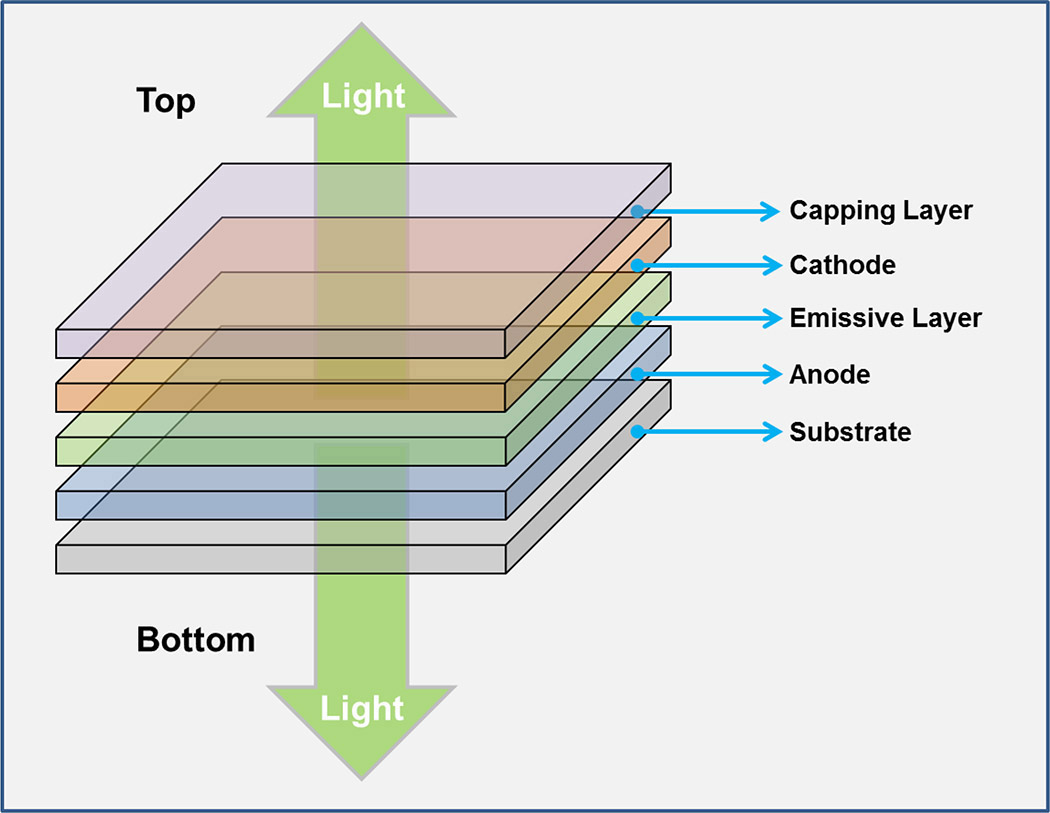
\includegraphics{figs/oled.jpg}
   \caption{Schematic diagram of OLED based on layered material showing how a functional device can be created from the combination of multiple layers that form an active region. At least one of the electrode layers in the device is made from a transparent conductor. Graphene is an ideal candidate material for transparent conducting electrodes in organic electronic devices. Reproduced with permission from:
\emph{SPIE Newsroom} November 2013: ``Transparent organic LEDs for new lighting applications,"  Jaehyun Moon, Jin Woo Huh, Chul Wong Joo, Jun-Han Han, Jonghee Lee, Hye Yong Chu and Jeong-Ik Lee.}

  \label{oled-fig}
\end{figure}

Application of organic materials in electronic technology offers many promising characteristics. First and foremost, many organic materials can be produced quickly and cheaply when compared to standard silicon semiconductor technology. Materials such as pentacene derivatives, perlyene derivatives like PTCDA, and carbon nanotubes are all carbon based materials which can act as semiconductors, which is the role silicon normally plays in a device. All of these materials can be synthesized with relative ease in a standard organic chemistry lab.

Many organic materials adopt structures that make them flexible while still retaining important electronic properties. Graphene and other sheet like polymer materials can be used as lightweight flexible conductors. Graphene in particular offers numerous other unique electronic properties making it an ideal candidate for study in organic electronics and will be the focus of later discussion. Flexibility in electronic devices is a property that is unknown to standard silicon based electronics. Mobile display technology, in the future, may make use of organic materials to create lightweight flexible OLED displays. A primary aim in integrating organic materials into electronic devices is to reduce cost. Transparent electrodes are necessary in many devices but current materials are often cost prohibitive; organic materials offer a low cost lightweight alternative.

Photovoltaic devices can be thought of, in principle, as an LED working in reverse. Thus it's easy to foresee that photovoltaic devices can be constructed using organic materials. Indeed organic photovoltaic (OPV) devices using fullerenes are in production for over two decades \cite{all-carbon}. In fact, it is possible to create an OPV device using only carbon \cite{all-carbon}. Carbon based materials in OPV devices offer the ability to create novel device architectures by making use of the flexible nature of organic materials. Flexible solar panels will allow greater adoption of solar power in modern society by greatly increasing the number of areas that can house photovoltaic devices. Lightweight flexible electronics and photovoltaics offer great possibilities for both terrestrial electronic applications as well as those used in satellites and space flight missions.

Finally, the environmental aspect of using organic materials in everyday electronic devices offers great promise. Organic electronic devices can be more energy efficient, which is beneficial, however, the benefit goes further. The manufacturing process used to create the devices promises to be more eco-friendly when compared to today's methods of electronic device production.

The benefits of organic electronic devices, their impact on our society, and a vision for the future have been laid out by the participants of the 2012 Chemical Sciences and Society Summit (CS3), briefly summarized here \cite{cs3}:
\begin{enumerate}
\item
Organic electronic devices will do things that silicon-based electronics cannot do.

\item
Organic electronic devices will be more energy-efficient and eco-friendly.

\item
Organic electronic devices will be manufactured in a more resource-friendly and sustainable fashion.
\end{enumerate}
All of the above statements indicate how organic electronics can be integral in contributing to a more sustainable future for our society.

\section{Graphene}
Graphene is an allotrope of solid carbon consisting of a single layer of $sp^2$ hybridized carbon atoms arranged in a hexagonal two-dimensional crystalline lattice. First isolated in 2004, graphene was the first truly two-dimensional material isolated in a lab setting \cite{apsnews}. Previously 2D materials were theorized to be thermally unstable and thus believed to not exist in nature \cite{Geim}. Thus, the isolation of graphene sparked an explosion of research. The entirely new field of study, 2D materials, seeks to analyze the properties of 2D materials and search for other materials, which are, like graphene, thermodynamically stable in a 2D crystalline phase. These materials present a rich variety of interesting properties making them useful in novel electronic architectures. To clarify the terminology, the designation of a material as two-dimensional stems from the fact that the mathematics describing the symmetry of the crystal lattice is purely two-dimensional. Many materials labeled as two-dimensional may contain multiple layers of atoms but the lattice as a whole has two-dimensional symmetry.

The honeycomb structure of graphene arises from the electron orbital hybridization in the carbon atoms. The $sp^2$ hybridization occurs when a carbon atom is bonded to three other atoms; in the case of graphene, all atoms are carbon. The bond hybridization results from a mixing between a carbon $2s$ orbital and two carbon $2p$ orbitals. This creates a set of three hybrid bonds where the state of minimal overlap between adjacent bonds manifests with a $120^\circ$ bond separation. This structure suggests crystalline graphene exists as a single sheet of carbon atoms where the nearest neighbor distance is 1.42 {\AA} with the actual hexagonal lattice constant larger by a factor of $\sqrt{3}$ at 2.46 {\AA}.  A diagram of the graphene structure can be seen in Figure \ref{Graphene-Structure-Figure}.

One of the interesting aspects of the graphene crystal structure is the two-atom unit cell. The hexagonal unit cell is made by adjoining only next-nearest neighbor carbon atoms, which are separated by a distance of 2.46 {\AA}. This means that nearest-neighbor carbon atoms are distinct from one another, these atoms are frequently labeled as A/B carbon atoms.  The lower portion of Figure \ref{Graphene-Structure-Figure} displays this characteristic. From this viewpoint, the graphene lattice can be considered as built from two separate interpenetrating trigonal lattices. The two-atom unit cell has direct implications for the electronic properties of graphene, which will be discussed later.

\begin{figure}
    \centering 
        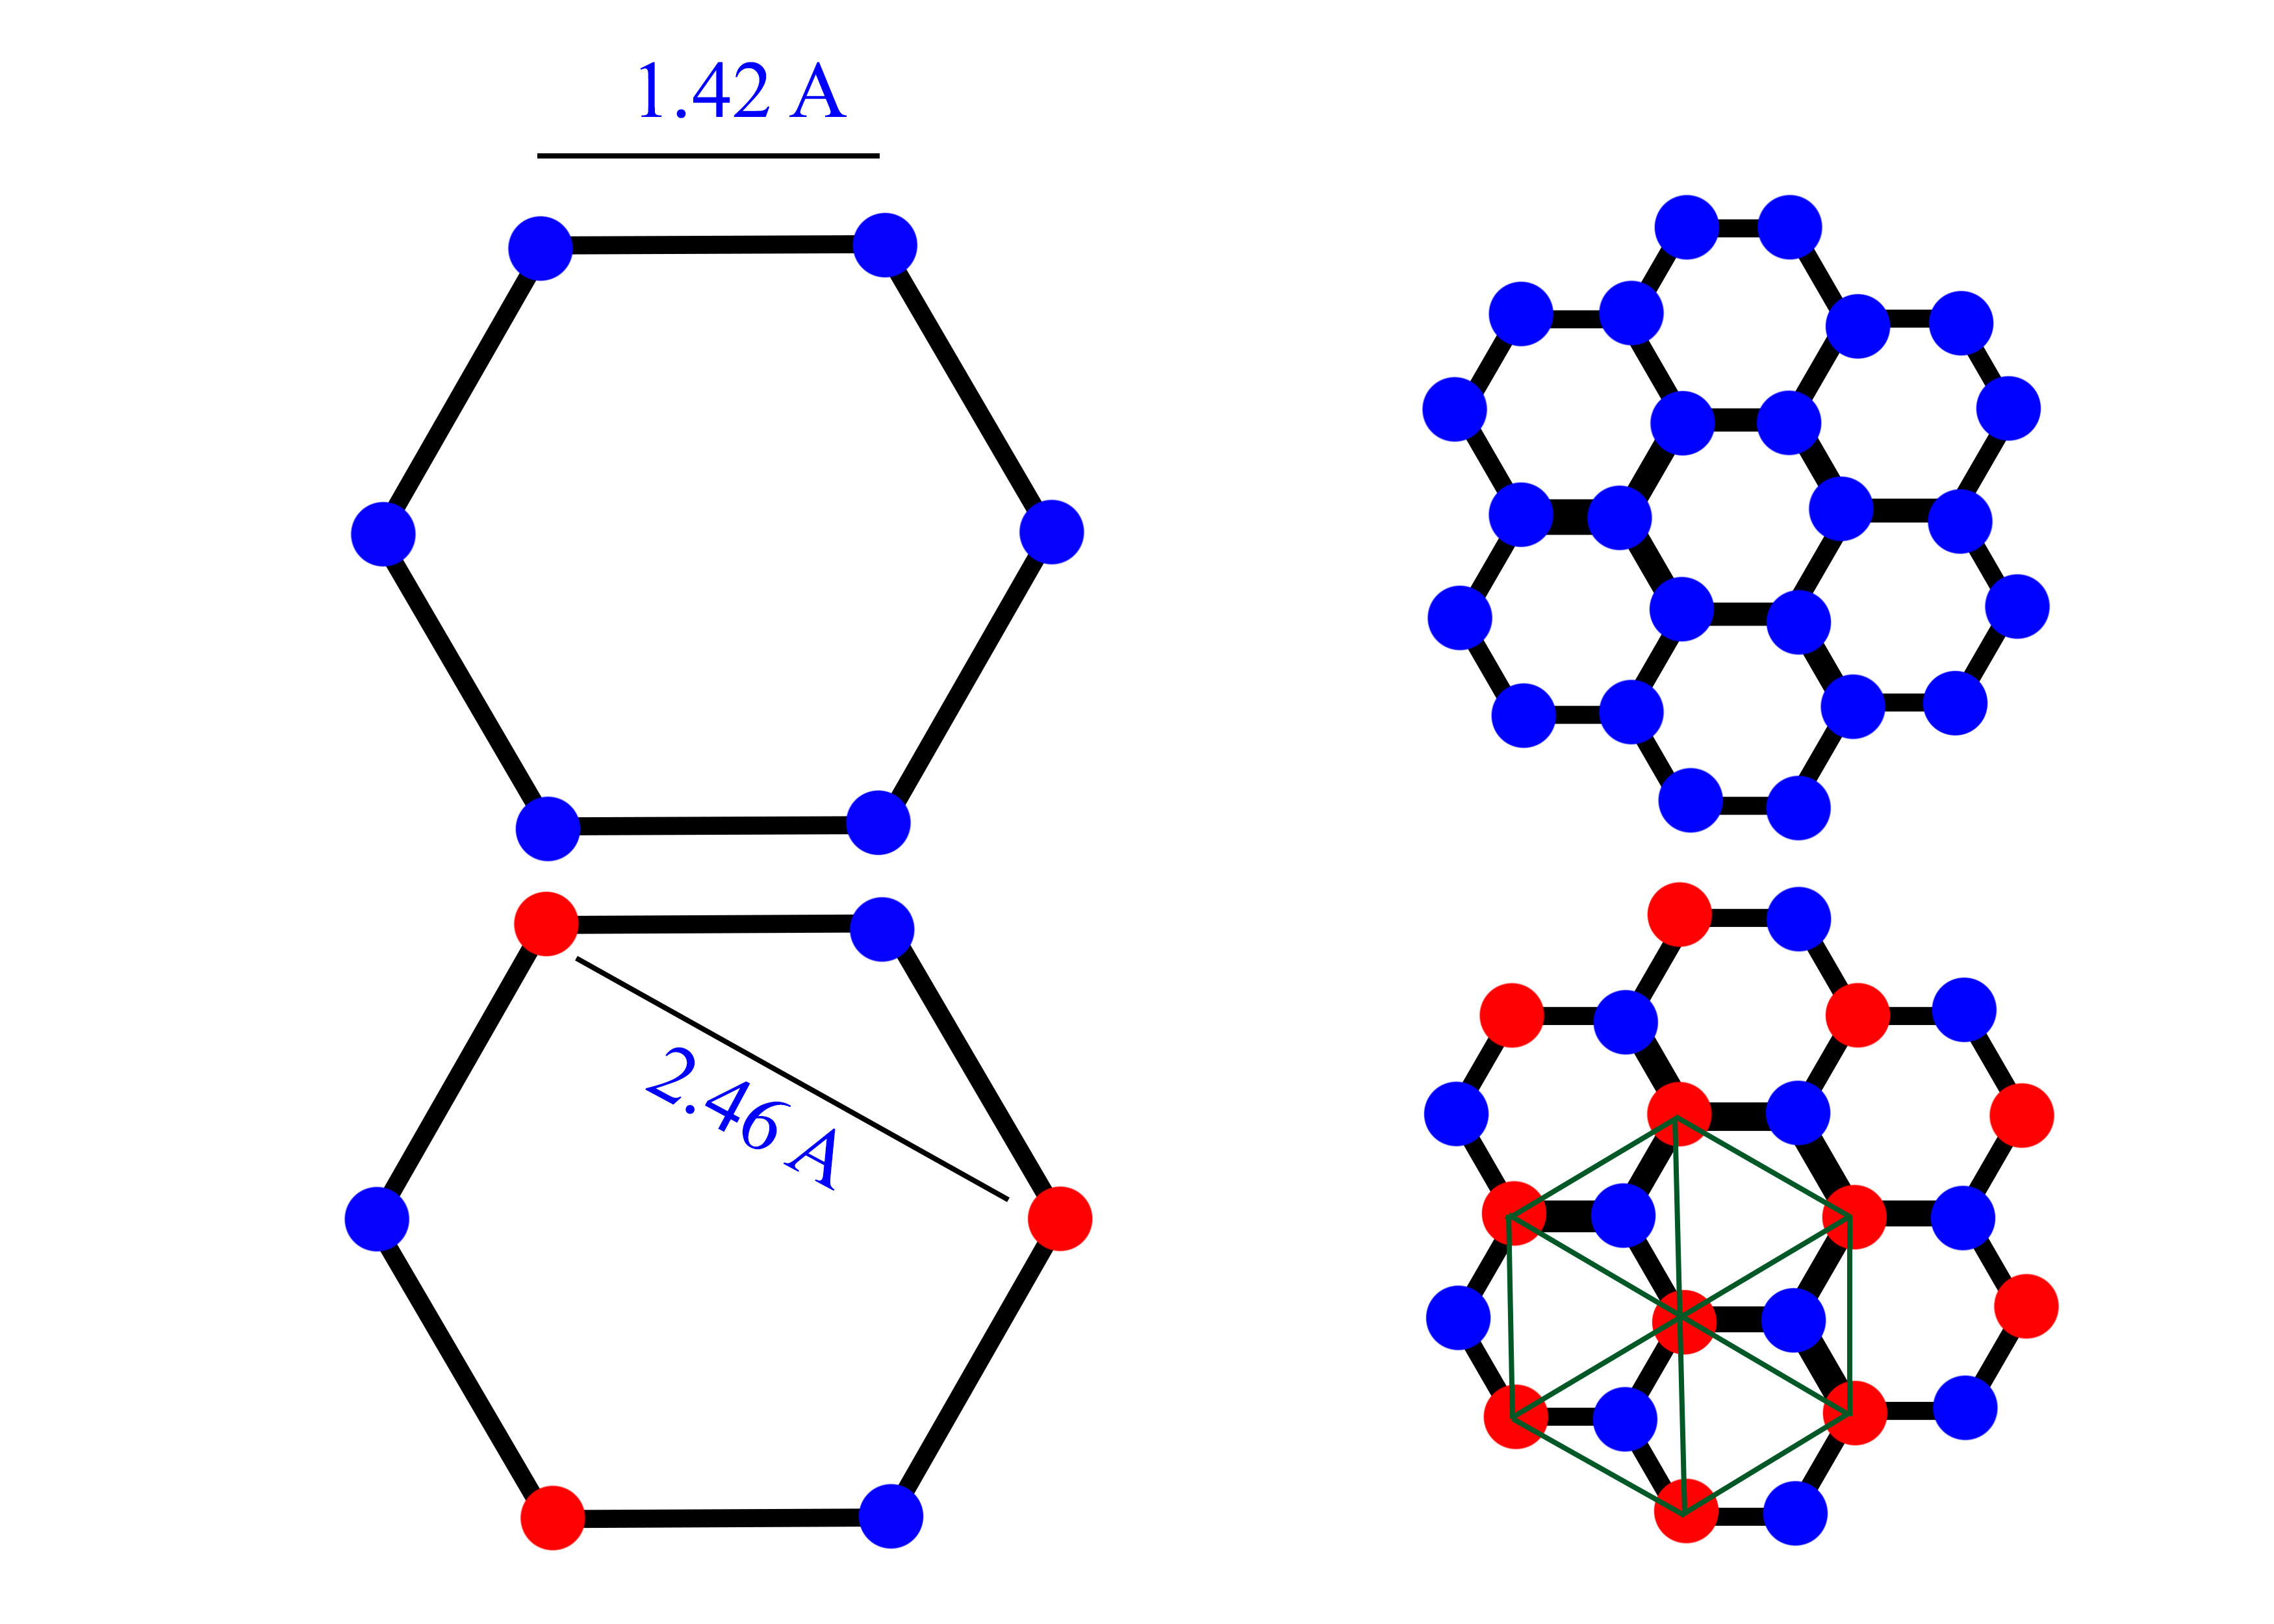
\includegraphics{figs/hexagonswithlength.jpg}
    \caption{Graphene honeycomb structure: (upper figure) 1.42 {\AA} nearest neighbor carbon distance. (lower figure) Characteristic two-atom unit cell: The nearest neighbor carbon atoms are distinct from each other and thus each graphene unit cell contains two atoms with lattice constant 2.46 {\AA}.
}
\label{Graphene-Structure-Figure}
\end{figure}

Soon after isolation, scientists studied and characterized numerous physical, optical, and electronic properties of the material. Graphene has a very high intrinsic electron mobility, in fact it has the highest mobility ever recorded \cite{Wolf}. A single sheet of graphene is nearly entirely transparent, only absorbing roughly 3\% of white light incident on the surface. This unique combination of high optical transparency with high electron mobility makes graphene an ideal candidate material for use as a transparent conductor in photovoltaic and light emitting devices such as OLED displays and flexible solar panels.

Currently, the material used in most devices in the role of a transparent conductor is indium tin oxide (ITO). Usage of ITO has a number of downsides. Namely, ITO is an expensive material to produce and apply in a device. The structure of ITO does not lend itself to flexibility without being incorporated into a polymer or nanofiber substrate, thus restricting device form factor. Finally, ITO, like many heavy metals, can cause health problems if inhaled or ingested which is a problem for recycling processes, and ITO also poses concerns for pollution in landfills.

Graphene has a wide variety of unique properties, many stemming directly from the 2D nature of the material. While graphene possesses a number of novel electronic properties, this doctoral work will focus primarily on the structural properties of graphene especially with regards to how the structure changes topology with respect different substrates. Finally the graphene surface structure will be analyzed from the viewpoint of a molecular scaffold for the self-assembly of atomic clusters and layers of organic semiconducting molecules.

\section{Self-Assembly}

It is often useful to think about nanoscale device fabrication from a top-down approach such as the familiar methods of etching devices into a silicon wafer via various lithographic techniques. However, another valid way to construct devices is to consider a bottom-up approach. Using this method, individual layers of materials are grown or deposited on a surface and combine to make an active region for a device in a layer-by-layer fashion. In order to improve device efficiency in a layered device, control over charge transport throughout and within the layers is of utmost importance.

When a material is grown or deposited onto a surface, the orientation of individual atoms or molecules within the material has a profound impact on the electronic properties of the material and thus on the device as a whole. The intermolecular forces combine with molecule-substrate forces to determine the overall topology of the layer. The strength of the intermolecular forces impacts the ability to transfer charge between molecules within a layer.

The growth process of a layer of molecules upon a crystalline surface is not guaranteed to produce a layer of material with any long-range intra-layer order. For example, consider analysis of the growth of derivatives of the prototypical organic semiconductor, pentacene, atop the gold (111) surface.  Scanning Tunneling Microscopy (STM) studies demonstrate with molecular resolution, that many phases of molecular packing relative to the gold surface coexist with poor long-range ordering \cite{wang-nano}. From a device standpoint, this inherent disorder within the pentacene layer is problematic. In the ideal scenario, all the pentacene molecules would adopt a single crystalline phase, thereby enhancing the ability to transfer charge between molecules within a layer.

There are a number of possible ways to address the issue of intra-layer order in a layered device. For example, many organic molecules provide a nearly endless amount of possible derivative molecules, which can be created or engineered by careful substitution of one atom or functional group for another. The addition of functional groups and substituent atoms to an organic molecule can have profound implications for not only the device characteristics but also the packing arrangement and preferred orientation of the molecule relative to the surface \cite{amanda-ttpo, bogdanc60}.

Outside of chemical functionalization, substrate modification provides another route towards guiding molecular orientation. Growth of pentacene derivatives on the stepped vicinal surface of gold (788) demonstrates the ability to create long-range intra-layer order within a monolayer of organic materials \cite{wang-nano}. The concept of surface structure modification as applied to growth of organic adsorbate layers and metallic clusters will be examined later with respect to the graphene surface.

The methods described above outline a process known as molecular self-assembly, the process through which molecules, atoms, or clusters of atoms or molecules adopt themselves into a well-defined arrangement without an external force to guide them into position. The ultimate goal of molecular self-assembly is to create new functional materials by assembling materials into an ordered supra-molecular device. Already many devices based on self-assembly have been created, such as bi-layer heterojunctions created from ordered organic semiconductors used in OLEDs and OPVs \cite{opv-self-assembly}. The latest advance in device design utilizing molecular self-assembly is the creation of a superconducting material by self-assembling a niobium-nitride in a matrix of organic block-copolymers. This marks the first superconducting device based on molecular self-assembly \cite{superconductor-self-assembly}.

Understanding molecular self-assembly requires an intuitive knowledge of the many forces that dictate molecular arrangement at the nanoscale. These forces can be strong forces such as those arising from the covalent bonding between adsorbate atoms and substrate atoms, however, often there are many very weak forces that much also be considered. Weak inter-molecular forces arising from dipole-dipole interactions, van der Waals interactions, and $\pi-\pi$ stacking are common in organic molecules and their contribution to molecular orientation cannot generally be overlooked. The presence of long-range weak forces also poses a problem for computational modeling of many organic molecules using density functional theory.

The UNH surface science lab has a rich history of preparation and analysis of a wide range of nanoscale molecular systems ranging from metallic nanoclusters to layered organic semiconductor heterojunctions. Previous work with fullerenes and pentacenes on gold and silver substrates has demonstrated the ability to engineer order within a molecular layer \cite{bogdan-sulfur, bogdanc60, wang, wang-nano, amanda-ttpo}. My doctoral work with graphene seeks to extend previous work with classic organic materials and metallic substrates and apply the same principles to a graphene system that possesses a novel surface structure.

\section{Surface Science}
The UNH surface science lab is uniquely equipped to probe the fundamental physics of the nanoscale world that takes place at the surface or interface between surfaces of a variety of novel materials. The primary reason surfaces are of interest is due to the fact that they represent a unique departure from the periodicity of three-dimensional materials. Surfaces represent a broken symmetry in one direction of an otherwise perfectly periodic solid material. This implies the atoms at the surface are distinct from atoms in the bulk material as they have a lower coordination number and thus often a higher chemical reactivity as well possibilities for localized quantum states not found in bulk.

Surface physics is crucial to understanding atomic reconstruction in solid crystals, epitaxial growth of layered materials, surface states and plasmons, as well as molecular self-assembly among many other topics. Knowledge of surface and interface physics is important for understanding many physical and chemical processes such as catalysis, photovoltaic energy production, oxidation and, corrosion. The study of catalysis is likely the original motivation for research in surface science however the driving factor in the modern explosion of surface science research is fabrication of semiconductor devices \cite{SurfSciTechniques}. The characterization of semiconductor surfaces, in general, requires detailed knowledge of atomic reconstruction relative to the bulk structure. Examples of this can be seen in the complex surface reconstructions of silicon and silicon carbide. Thus to adequately understand physics at the surface, tools for discerning precise atomic positions are needed \cite{SurfSciTechniques}.

In order to study surfaces at a fundamental level, a pristine environment is required to preserve the atomic composition over significant time scales. Thus much work in surface science and all work in this thesis takes place in an ultra high vacuum (UHV) environment. In UHV, a surface prepared for an experiment can be considered clean or well characterized for many hours before any significant contamination has built up. This leaves ample time for surface sensitive experiments to take place.

The primary work this thesis utilizes for surface analysis is scanning tunneling microscopy (STM). STM is a non-optical form of microscopy using a scanning metallic probe and quantum tunneling to extract data and generate images of the local density of electronic states at the surface. Quantum tunneling has no classical analog and is a physical phenomenon restricted solely to the nanoscale regime.

STM is a powerful tool for probing the real space structure of surfaces with unmatched resolution in all directions. While the data directly produced by an STM is a map of the local density of states in the surface, from this data the exact positions of atoms in the material can be extracted. Thus STM provides a way to map the topography of the surface with atomic resolution, something impossible with optical microscopy due to the diffraction limit of visible light. The ultra-high resolution provided by STM is extremely important for the study of molecular self-assembly and atomic reconstructions. The microscope used for much of my thesis work is a homebuilt variable temperature scanning tunneling microscope (VT-STM) housed in an ultra high vacuum chamber with an ultimate pressure better than $10^{-10}$ torr integrated with a number of other tools for surface preparation and analysis.

The second primary tool for surface analysis and preparation used in this thesis work is Low Energy Electron Diffraction (LEED). Whereas STM provides real space information about the surface with highly localized resolution, LEED provides momentum space information about the surface in a much larger sample area. Using LEED, the crystal structure of the surface region in a sample can be determined with relative ease. A related technique using the same LEED optics, Auger Electron Spectroscopy (AES) maps the surface elemental composition with a high degree of accuracy. LEED and AES together combine to make ideal tools for assessing and monitoring UHV sample preparation. The UHV system at UNH used for this thesis work is equipped with an Omicron SpectaLEED rear view LEED/AES system.

The reciprocal space images generated by LEED give qualitative information on how well ordered the sample surface is from a crystallographic standpoint. A well ordered single crystal surface has sharp precise diffraction maxima in reciprocal space whereas a sample with multiple domains or rotational disorder has diffuse diffraction maxima spread over a larger region in reciprocal space. The LEED pattern seen from a given surface represents a scaled version of the sample surface reciprocal lattice and contains information about rotational symmetries in the surface.

One of the major restrictions for conventional LEED systems is the beam geometry with respect to the sample blocking view of the spectrally reflected beam. At very low energies, all higher order beams exist at diffraction angles too large to be imaged. Since the spectral beam is blocked by the electron source, conventional LEED has a minimum energy in the 40-60 eV range where no data can be collected for incident beam energies lower than this threshold.

Of interest to the study of this novel graphene system are the interactions between very low energy electrons and layered surfaces and thin films. Very low energy electrons, E $<$ 20 eV, have unique interactions with thin films due to quantum confinement effects. These effects manifest as oscillations in the electron reflectivity curves. It has been shown previously that these oscillations can be used to map the layer thickness in thin films such as metallic monolayers or graphene layers \cite{Hannon-LEEM-Book}. To bypass the minimum energy restriction of conventional LEED systems, I utilize a third surface science technique called low energy electron microscopy (LEEM).

LEEM instruments are a subset of cathode lens microscopes, where the sample being probed is held at high negative potential and acts as part of the lens system itself. LEEM systems allow many different beam line geometries compared to conventional LEED through the use of magnetic prism arrays. This allows all reflected beams to be imaged simultaneously and also allows for imaging of the surface while a dynamic process such as epitaxial growth takes place. LEEM can also easily collect data at very low incident electron energy, thus the restriction of minimum energy from conventional LEED is lifted.

What separates LEEM primarily from LEED, however, are not just alternate geometries and energy ranges. Rather, LEEM can operate in both real space imaging mode and reciprocal space imaging mode and can switch between the two quite rapidly simply by swapping which optical plane is projected into the detection column. Thus a surface can be imaged with resolution on the order of a few nanometers in real space and without much effort, the same area of the sample can then be probed in reciprocal space using LEED techniques. Furthermore, the size of the area probed using LEED mode can be restricted well below that possible in conventional LEED setups. A LEEM instrument  allows LEED data to be collected from a selected area in the real space image using special contrast apertures added to the beam line. The combined ability to acquire high resolution real space surface images with localized reciprocal space data makes LEEM an incredibly powerful tool for surface sensitive studies.   

Finally, both LEEM and LEED experiments can provide three-dimensional information regarding the crystal structure near the surface region of the sample. While analysis of static LEED patterns provides information in the two-dimensional surface plane, additional three-dimensional information can be accessed using a technique called LEED/LEEM-I(V). By varying the energy of the incident electron beam and recording the intensity of the reflected or diffracted electrons, one can analyze how the electron reflectivity depends on energy. The shape of these electron reflectivity curves provides information about the three-dimensional atomic structure of the surface. This technique, however, requires close collaboration with theoretical modeling of the surface in order to fit the experimental curves to those predicted by theory.

To aid in the analysis of LEED and LEEM-I(V) data sets, I have designed a software package using python to visualize LEED and LEEM data and allow quick and reproducible extraction of I(V) curves. This software is currently being used to help with I(V) studies of numerous two-dimensional materials through collaboration external research groups. Analysis of LEEM-I(V) data from our graphene system will provide additional information about the system not easily achievable with STM or conventional LEED alone.

\section{Summary}
This thesis outlines research into a variety of novel materials for future application in electronic devices based on layered 2D materials. 
	My work focuses on the structural properties of a novel polymorphic graphene system, developed at UNH, which presents a unique structure that can be utilized as a template for molecular self-assembly. Control over the growth of clusters of metals and organic semiconducting molecules will be important to future work in enhancing efficiency in nanoscale electronic devices. Understanding the underlying physics, which governs charge transfer both within as well as between material layers in a nanoscale device, will be crucial to characterization of device parameters. Specifically, for organic electronic devices, it is important to understand how device structure and morphology affects processes such as diffusive charge transport, exciton recombination, and charge collection at electrodes.
	The materials discussed in this work have potential for use in a wide array of electronic devices from photovoltaic applications to organic electronic lighting and from highly sensitive chemical sensors to touch screen displays. Terrestrial applications of organic electronics are not the only market standing to benefit from advances in the field. Organic electronics and organic photovoltaics are also of great interest for satellite design and space flight missions to reduce cost, enhance power generation, and increase the overall efficiency of devices onboard.

\begin{itemize}
\item Chapter 1, \emph{Introduction} 
\item Chapter 2, \emph{Graphene}
\item Chapter 3, \emph{Tools for Surface Science}
\item Chapter 4, \emph{Polymorphic Graphene: modulating the graphene surface structure}
\item Chapter 5, \emph{LEEM/LEED-I(V) study of two-dimensional materials}
\item Chapter 6 \emph{Conclusions}
\end{itemize}

% ------------------- %